%% Public domain image from
%% http://www.public-domain-image.com/still-life/slides/cherry-tomatos.html

\renewcommand\chapterillustration{cherry-tomatos}
\chapter{文件系统中跳转}

我们需要学习的第一件事(除了打字之外)是如何在 Linux 文件系统中跳转。 在这一章节中,我们将介绍以下命令:
\begin{itemize}
	\item pwd — 打印出当前工作目录名
	\item cd — 更改目录
	\item ls — 列出目录内容
\end{itemize}



\section{理解文件系统树} % (fold)
\label{sec:理解文件系统树}

正如 Windows,一个类似于 Unix 的操作系统,比如说 Linux,以分层目录结构来组织所有文件。 这就意味着所有文件组成了一棵树型目录(有时候在其它系统中叫做文件夹), 这个目录树可能包含文件和其它的目录。文件系统中的第一级目录称为根目录。 根目录包含文件和子目录,子目录包含更多的文件和子目录,依此类推。

\par 注意不同于 Windows,Windows 每个存储设备都有一个独自的文件系统,类似于 Unix 的操作系统, 比如说 Linux,总是有一个单一的文件系统树,不管有多少个磁盘或者存储设备连接到计算机上。 根据系统管理员的兴致,存储设备连接到(或着更精确些,是挂载到)目录树的各个节点上。 系统管理员负责维护系统安全。


% section 理解文件系统树 (end)

\section{当前工作目录}

\begin{figure}[h!]
\centering
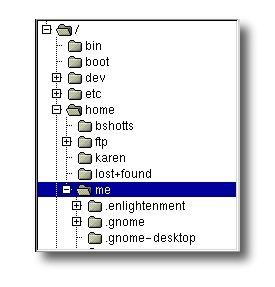
\includegraphics[width=2.5in]{images/1.png}
\caption{File system tree as shown by a graphical file manager}
\label{fig_sim}
\end{figure}

大多数人都可能熟悉图形文件管理器,它描述了文件系统树的结构,正如图1所示。 注意通常,这是一棵倒置的树,也就是说,树根在最上面,而各个枝干在下面展开。

\par 然而,命令行没有图片,所以我们需要考虑用不同的方法,在文件系统树中跳转。

\par 把文件系统想象成一个迷宫形状,就像一棵倒立的大树,我们站在迷宫的中间位置。 在任意时刻,我们处于一个目录里面,我们能看到这个目录包含的所有文件, 以及通往上面目录(父目录)的路径,和下面的各个子目录。我们所在的目录则称为 当前工作目录。我们使用 pwd(打印工作目录)命令,来显示当前工作目录。

\begin{lstlisting}
[me@linuxbox ~]$ pwd
/home/me
\end{lstlisting}

\par 当我们首次登录系统后,(或者启动终端仿真器会话后),当前工作目录设置成主目录。 每个用户都有他自己的主目录,当用户以普通用户的身份操控系统时,主目录是唯一 允许用户编写文件的地方。



\section{列出目录内容} % (fold)
\label{sec:列出目录内容}

列出一个目录包含的文件及子目录,使用 ls 命令。

\begin{lstlisting}
[me@linuxbox ~]$ ls
Desktop Documents Music Pictures Public Templates Videos
\end{lstlisting}

\par 实际上,用 ls 命令可以列出任一个目录的内容,而不只是当前工作目录的内容。 ls 命令还能完成许多有趣的事情。在下一章节,我们将介绍更多关于 ls 的知识。
% section 列出目录内容 (end)

\section{更改当前工作目录} % (fold)
\label{sec:更改当前工作目录}
\par 要更改工作目录(此刻,我们站在树形迷宫里面),我们用 cd 命令。输入 cd, 然后输入你想要的工作目录的路径名,就能实现愿望。路径名就是沿着目录树的分支 到达想要的目录,期间所经过的路线。路径名可通过两种方式来指定,一个是绝对路径, 另一个是相对路径。首先处理绝对路径。

\subsection{绝对路径} % (fold)
\label{ssub:绝对路径}
绝对路径开始于根目录,紧跟着目录树的一个个分支,一直到达期望的目录或文件。 例如,你的系统中有一个目录,大多数系统程序都安装在这个目录下。这个目录的 路径名是 /usr/bin。它意味着从根目录(用开头的“/”表示)开始,有一个叫 “usr” 的 目录包含了目录 “bin”。
\begin{lstlisting}
[me@linuxbox ~]$ cd /usr/bin
[me@linuxbox bin]$ pwd
/usr/bin
[me@linuxbox bin]$ ls
...Listing of many, many files ...
\end{lstlisting}
\par 我们把工作目录转到 /usr/bin 目录下,里面装满了文件。注意 shell 提示符是怎样改变的。 为了方便,通常设置提示符自动显示工作目录名。
% subsection 绝对路径 (end)

\subsection{相对路径} % (fold)
\label{sub:相对路径}
绝对路径从根目录开始,直到它的目的地,而相对路径开始于工作目录。 一对特殊符号来表示相对位置,在文件系统树中。这对特殊符号是 ``.'' (点) 和 ``..'' (点点)。

\par 符号 ``.'' 指的是工作目录,``..'' 指的是工作目录的父目录。下面的例子说明怎样使用它。 再次更改工作目录到 /usr/bin:
\begin{lstlisting}
[me@linuxbox ~]$ cd /usr/bin
[me@linuxbox bin]$ pwd
/usr/bin
\end{lstlisting}

\par 好的,比方说更改工作目录到 /usr/bin 的父目录 /usr。可以通过两种方法来实现。或者使用绝对路径名:

\begin{lstlisting}
[me@linuxbox bin]$ cd /usr
[me@linuxbox usr]$ pwd
/usr
\end{lstlisting}

\par 或者, 使用相对路径:

\begin{lstlisting}
[me@linuxbox bin]$ cd ..
[me@linuxbox usr]$ pwd
/usr
\end{lstlisting}

\par 两种不同的方法,一样的结果。我们应该选哪一个呢? 输入量最少的那个。

\par 同样地,从目录/usr/到/usr/bin 也有两种途径。或者使用绝对路径:

\begin{lstlisting}
[me@linuxbox usr]$ cd /usr/bin
[me@linuxbox bin]$ pwd
/usr/bin
\end{lstlisting}

\par 或者,用相对路径:

\begin{lstlisting}
[me@linuxbox usr]$ cd ./bin
[me@linuxbox bin]$ pwd
/usr/bin
\end{lstlisting}

\par 有一件很重要的事,我必须指出来。在几乎所有的情况下,你可以省略”./”。它是隐含地。输入:
\begin{lstlisting}
[me@linuxbox usr]$ cd bin
\end{lstlisting}

\par 实现相同的效果,如果不指定一个文件的目录,那它的工作目录会被假定为当前工作目录。

% subsection 相对路径 (end)

\subsubsection{有用的快捷键} % (fold)
\label{ssub:有用的快捷键}
在表2-1中,列举出了一些快速改变当前工作目录的有效方法。


\begin{table}[ht!]
% increase table row spacing, adjust to taste
%\renewcommand{\arraystretch}{1.2}
\caption{cd 快捷键}
\label{table_example}
\centering
\begin{tabular}{c|c}
\hline
%\begin{tabular}{|p{0.18\textwidth}|p{0.36\textwidth}|p{0.36\textwidth}|}
 快捷键 & 运行结果 \\
\hline
  cd	& 更改工作目录到主目录。 \\
  cd -	& 更改工作目录到先前的工作目录。\\
cd ~user\_name	& 更改工作目录到用户主目录。例如, cd ~bob 会更改工作目录到用户“bob”的主目录。\\
\hline
\end{tabular}
\end{table}

% subsubsection 有用的快捷键 (end)
\fboxrule=6pt \fboxsep=4pt
\begin{colorboxed}[boxcolor=lightgray,bgcolor=white]
\subsubsection{关于文件名的重要规则}
\begin{enumerate}
	\item 以 ``.'' 字符开头的文件名是隐藏文件。这仅表示,ls 命令不能列出它们, 除非使用 ls -a 命令。当你创建帐号后,几个配置帐号的隐藏文件被放置在 你的主目录下。稍后,我们会仔细研究一些隐藏文件,来定制你的系统环境。 另外,一些应用程序也会把它们的配置文件以隐藏文件的形式放在你的主目录下面。
	\item 文件名和命令名是大小写敏感的。文件名 “File1” 和 “file1” 是指两个不同的文件名。
	\item Linux 没有“文件扩展名”的概念,不像其它一些系统。可以用你喜欢的任何名字 来给文件起名。文件内容或用途由其它方法来决定。虽然类似 Unix 的操作系统, 不用文件扩展名来决定文件的内容或用途,但是应用程序会。
	\item 虽然 Linux 支持长文件名,文件名可能包含空格,标点符号,但标点符号仅限 使用 ``.'',``-'',下划线。最重要的是,不要在文件名中使用空格。如果你想表示词与 词间的空格,用下划线字符来代替。过些时候,你会感激自己这样做。
\end{enumerate}
\end{colorboxed}
% section 更改当前工作目录 (end)

